%%%%%%%%%%%%%%%%%%%%%%%%%%%%%%%%%%%%%%%%%%%%%%%%%%%%%%%%%%%%%%%%%%%%%%%%%%%%%%%%%
%
% Purpose:  Conceptual part of Product Spec for the Relative model
%
% 
%
%%%%%%%%%%%%%%%%%%%%%%%%%%%%%%%%%%%%%%%%%%%%%%%%%%%%%%%%%%%%%%%%%%%%%%%%%%%%%%%%


%\section{Conceptual Design}

The \RelativeDesc\ provides the state of one vehicle with respect to some other reference frame (often associated with another vehicle, but not necessarily so).  The two reference frames (the vehicle's reference frame and the other reference frame) are labeled \textit{subject} and \textit{target}.  This model is sufficiently flexible to represent the state of either reference frame with respect to the other.  As of version 3.4, the \textit{subject} frame no longer must be associated with a Dynamic Body, but can be any arbitrary frame in the simulation.  However, the model is fully backwards compatible to the previous usage when it was required to be associated with a Dynamic Body. The \textit{target} never had the Dynamic Body restriction. The original intent was that the subject of the relative state calculation be a vehicle, while the target could be a planet, or some defined point unassociated with any mass, though in actuality the calculation is the same regardless of the nature of the reference frame's owning point or model. The updated capability reflects this.

When expressing the state of some frame, \textit{A} with respect to some other frame, \textit{B}, the tranlational position and velocity are expressed in frame \textit{B}, while the angular velocity is expressed in frame \textit{A}; the angular position (expressed as a quaternion or transformation matrix) is frame-independent.

As a simple example, consider two reference frames, \textit{S} and \textit{S'}.  Suppose that \textit{S'} is moving with some velocity \textit{u} along the x-axis of reference frame \textit{S}, and has its origin momentarily located at $(x_0,y_0)$  Consider further that \textit{S'} is rotated by ninety degrees about the z-axis from \textit{S}, so that $x' = y,  y' = -x, z' = z$.  An illustration is shown in Figure~\ref{fig:relstatereforient}.

\begin{figure}[ht]
\begin{center}
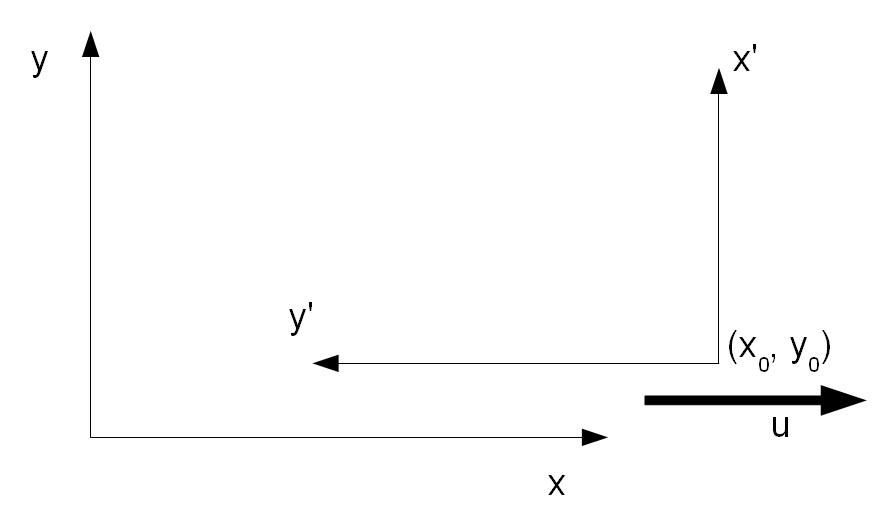
\includegraphics[width=3.5in]{figures/rel_state_ref_orient.jpg}
\caption{The momentary positions, velocity, and orientation of frames \textit{S} and \textit{S'}}
\label{fig:relstatereforient}
\end{center}
\end{figure}

There are four ways of expressing this relation:  the state of \textit{S'} can be expressed with respect to \textit{S}, or \textit{S} with respect to \textit{S'}; for each case, the result could be expressed in \textit{S} or in \textit{S'}.  In this example, the state of  \textit{S'} with respect to \textit{S}, can be represented as 

\begin{align*}
\vec x_{S'|S:S} & = (x_0, y_0) \\ 
\vec v_{S'|S:S} & = (u,0)\\
\vec x_{S'|S:S'} & = (y_0, -x_0) \\
\vec v_{S'|S:S'} & = (0,-u)
\end{align*}

where $ \vec x_{A|B:C}$ is the position of A with respect to B, expressed in C.

Similarly, the state of  \textit{S} with respect to \textit{S'}, can be represented as 

\begin{align*}
\vec x_{S\_S':S} & = (-x_0, -y_0) \\
\vec v_{S\_S':S} & = (-u,0)\\
\vec x_{S\_S':S'} & = (-y_0, x_0)\\
\vec v_{S\_S':S'} & = (0,u)
\end{align*}

Thus, the relative position (or velocity) could be described in four ways, using just these two frames.  Of these four representations, this model can provide $\vec x_{S'|S:S}$ and $\vec x_{S\_S':S'}$.

To make the system completely generic, the usage of \textit{subject} and \textit{target} are, for the most part, just names.  The \RelativeDesc\ will calculate the state of either with respect to the other.  Hence, in the example above, S and S' can be interchangeably identified as \textit{subject} and \textit{target}.  Again, the only restriction on assigning the \textit{subject} and \textit{target} is that the \textit{subject} must be associated with a Dynamic Body.

The user must specify three quantities:
\begin{itemize}
\item{Subject reference frame (by name)}
\item{Target reference frame (by name)}
\item{Sense in which to interpret the request}
\end{itemize}

the latter item in this list can be one of the two values described above:
\begin{itemize}
\item{Subject with respect to Target, expressed in Target (ComputeSubjectStateinTarget)}
\item{Target with respect to Subject, expressed in Subject (ComputeTargetStateinSubject)}
\end{itemize}

Note that this description is intended to convey information on the translational state only.  The angular velocity of the Subject frame will be expressed in the Subject frame, and the angular velocity of the Target frame will be expressed in the target frame.  The expression of the relative orientations of the two frames is frame independent.
